% Options for packages loaded elsewhere
\PassOptionsToPackage{unicode}{hyperref}
\PassOptionsToPackage{hyphens}{url}
\PassOptionsToPackage{dvipsnames,svgnames,x11names}{xcolor}
%
\documentclass[
  12pt,
  letterpaper,
  DIV=11,
  numbers=noendperiod]{scrartcl}

\usepackage{amsmath,amssymb}
\usepackage{iftex}
\ifPDFTeX
  \usepackage[T1]{fontenc}
  \usepackage[utf8]{inputenc}
  \usepackage{textcomp} % provide euro and other symbols
\else % if luatex or xetex
  \usepackage{unicode-math}
  \defaultfontfeatures{Scale=MatchLowercase}
  \defaultfontfeatures[\rmfamily]{Ligatures=TeX,Scale=1}
\fi
\usepackage{lmodern}
\ifPDFTeX\else  
    % xetex/luatex font selection
\fi
% Use upquote if available, for straight quotes in verbatim environments
\IfFileExists{upquote.sty}{\usepackage{upquote}}{}
\IfFileExists{microtype.sty}{% use microtype if available
  \usepackage[]{microtype}
  \UseMicrotypeSet[protrusion]{basicmath} % disable protrusion for tt fonts
}{}
\makeatletter
\@ifundefined{KOMAClassName}{% if non-KOMA class
  \IfFileExists{parskip.sty}{%
    \usepackage{parskip}
  }{% else
    \setlength{\parindent}{0pt}
    \setlength{\parskip}{6pt plus 2pt minus 1pt}}
}{% if KOMA class
  \KOMAoptions{parskip=half}}
\makeatother
\usepackage{xcolor}
\setlength{\emergencystretch}{3em} % prevent overfull lines
\setcounter{secnumdepth}{3}
% Make \paragraph and \subparagraph free-standing
\ifx\paragraph\undefined\else
  \let\oldparagraph\paragraph
  \renewcommand{\paragraph}[1]{\oldparagraph{#1}\mbox{}}
\fi
\ifx\subparagraph\undefined\else
  \let\oldsubparagraph\subparagraph
  \renewcommand{\subparagraph}[1]{\oldsubparagraph{#1}\mbox{}}
\fi

\usepackage{color}
\usepackage{fancyvrb}
\newcommand{\VerbBar}{|}
\newcommand{\VERB}{\Verb[commandchars=\\\{\}]}
\DefineVerbatimEnvironment{Highlighting}{Verbatim}{commandchars=\\\{\}}
% Add ',fontsize=\small' for more characters per line
\usepackage{framed}
\definecolor{shadecolor}{RGB}{241,243,245}
\newenvironment{Shaded}{\begin{snugshade}}{\end{snugshade}}
\newcommand{\AlertTok}[1]{\textcolor[rgb]{0.68,0.00,0.00}{#1}}
\newcommand{\AnnotationTok}[1]{\textcolor[rgb]{0.37,0.37,0.37}{#1}}
\newcommand{\AttributeTok}[1]{\textcolor[rgb]{0.40,0.45,0.13}{#1}}
\newcommand{\BaseNTok}[1]{\textcolor[rgb]{0.68,0.00,0.00}{#1}}
\newcommand{\BuiltInTok}[1]{\textcolor[rgb]{0.00,0.23,0.31}{#1}}
\newcommand{\CharTok}[1]{\textcolor[rgb]{0.13,0.47,0.30}{#1}}
\newcommand{\CommentTok}[1]{\textcolor[rgb]{0.37,0.37,0.37}{#1}}
\newcommand{\CommentVarTok}[1]{\textcolor[rgb]{0.37,0.37,0.37}{\textit{#1}}}
\newcommand{\ConstantTok}[1]{\textcolor[rgb]{0.56,0.35,0.01}{#1}}
\newcommand{\ControlFlowTok}[1]{\textcolor[rgb]{0.00,0.23,0.31}{#1}}
\newcommand{\DataTypeTok}[1]{\textcolor[rgb]{0.68,0.00,0.00}{#1}}
\newcommand{\DecValTok}[1]{\textcolor[rgb]{0.68,0.00,0.00}{#1}}
\newcommand{\DocumentationTok}[1]{\textcolor[rgb]{0.37,0.37,0.37}{\textit{#1}}}
\newcommand{\ErrorTok}[1]{\textcolor[rgb]{0.68,0.00,0.00}{#1}}
\newcommand{\ExtensionTok}[1]{\textcolor[rgb]{0.00,0.23,0.31}{#1}}
\newcommand{\FloatTok}[1]{\textcolor[rgb]{0.68,0.00,0.00}{#1}}
\newcommand{\FunctionTok}[1]{\textcolor[rgb]{0.28,0.35,0.67}{#1}}
\newcommand{\ImportTok}[1]{\textcolor[rgb]{0.00,0.46,0.62}{#1}}
\newcommand{\InformationTok}[1]{\textcolor[rgb]{0.37,0.37,0.37}{#1}}
\newcommand{\KeywordTok}[1]{\textcolor[rgb]{0.00,0.23,0.31}{#1}}
\newcommand{\NormalTok}[1]{\textcolor[rgb]{0.00,0.23,0.31}{#1}}
\newcommand{\OperatorTok}[1]{\textcolor[rgb]{0.37,0.37,0.37}{#1}}
\newcommand{\OtherTok}[1]{\textcolor[rgb]{0.00,0.23,0.31}{#1}}
\newcommand{\PreprocessorTok}[1]{\textcolor[rgb]{0.68,0.00,0.00}{#1}}
\newcommand{\RegionMarkerTok}[1]{\textcolor[rgb]{0.00,0.23,0.31}{#1}}
\newcommand{\SpecialCharTok}[1]{\textcolor[rgb]{0.37,0.37,0.37}{#1}}
\newcommand{\SpecialStringTok}[1]{\textcolor[rgb]{0.13,0.47,0.30}{#1}}
\newcommand{\StringTok}[1]{\textcolor[rgb]{0.13,0.47,0.30}{#1}}
\newcommand{\VariableTok}[1]{\textcolor[rgb]{0.07,0.07,0.07}{#1}}
\newcommand{\VerbatimStringTok}[1]{\textcolor[rgb]{0.13,0.47,0.30}{#1}}
\newcommand{\WarningTok}[1]{\textcolor[rgb]{0.37,0.37,0.37}{\textit{#1}}}

\providecommand{\tightlist}{%
  \setlength{\itemsep}{0pt}\setlength{\parskip}{0pt}}\usepackage{longtable,booktabs,array}
\usepackage{calc} % for calculating minipage widths
% Correct order of tables after \paragraph or \subparagraph
\usepackage{etoolbox}
\makeatletter
\patchcmd\longtable{\par}{\if@noskipsec\mbox{}\fi\par}{}{}
\makeatother
% Allow footnotes in longtable head/foot
\IfFileExists{footnotehyper.sty}{\usepackage{footnotehyper}}{\usepackage{footnote}}
\makesavenoteenv{longtable}
\usepackage{graphicx}
\makeatletter
\def\maxwidth{\ifdim\Gin@nat@width>\linewidth\linewidth\else\Gin@nat@width\fi}
\def\maxheight{\ifdim\Gin@nat@height>\textheight\textheight\else\Gin@nat@height\fi}
\makeatother
% Scale images if necessary, so that they will not overflow the page
% margins by default, and it is still possible to overwrite the defaults
% using explicit options in \includegraphics[width, height, ...]{}
\setkeys{Gin}{width=\maxwidth,height=\maxheight,keepaspectratio}
% Set default figure placement to htbp
\makeatletter
\def\fps@figure{htbp}
\makeatother

\usepackage{booktabs}
\usepackage{longtable}
\usepackage{array}
\usepackage{multirow}
\usepackage{wrapfig}
\usepackage{float}
\usepackage{colortbl}
\usepackage{pdflscape}
\usepackage{tabu}
\usepackage{threeparttable}
\usepackage{threeparttablex}
\usepackage[normalem]{ulem}
\usepackage{makecell}
\usepackage{xcolor}
\KOMAoption{captions}{tableheading}
\makeatletter
\@ifpackageloaded{caption}{}{\usepackage{caption}}
\AtBeginDocument{%
\ifdefined\contentsname
  \renewcommand*\contentsname{Table of contents}
\else
  \newcommand\contentsname{Table of contents}
\fi
\ifdefined\listfigurename
  \renewcommand*\listfigurename{List of Figures}
\else
  \newcommand\listfigurename{List of Figures}
\fi
\ifdefined\listtablename
  \renewcommand*\listtablename{List of Tables}
\else
  \newcommand\listtablename{List of Tables}
\fi
\ifdefined\figurename
  \renewcommand*\figurename{Figure}
\else
  \newcommand\figurename{Figure}
\fi
\ifdefined\tablename
  \renewcommand*\tablename{Table}
\else
  \newcommand\tablename{Table}
\fi
}
\@ifpackageloaded{float}{}{\usepackage{float}}
\floatstyle{ruled}
\@ifundefined{c@chapter}{\newfloat{codelisting}{h}{lop}}{\newfloat{codelisting}{h}{lop}[chapter]}
\floatname{codelisting}{Listing}
\newcommand*\listoflistings{\listof{codelisting}{List of Listings}}
\makeatother
\makeatletter
\makeatother
\makeatletter
\@ifpackageloaded{caption}{}{\usepackage{caption}}
\@ifpackageloaded{subcaption}{}{\usepackage{subcaption}}
\makeatother
\ifLuaTeX
\usepackage[bidi=basic]{babel}
\else
\usepackage[bidi=default]{babel}
\fi
\babelprovide[main,import]{english}
% get rid of language-specific shorthands (see #6817):
\let\LanguageShortHands\languageshorthands
\def\languageshorthands#1{}
\ifLuaTeX
  \usepackage{selnolig}  % disable illegal ligatures
\fi
\usepackage{bookmark}

\IfFileExists{xurl.sty}{\usepackage{xurl}}{} % add URL line breaks if available
\urlstyle{same} % disable monospaced font for URLs
\hypersetup{
  pdftitle={Data analysis},
  pdfauthor={Researcher},
  pdflang={en},
  colorlinks=true,
  linkcolor={blue},
  filecolor={Maroon},
  citecolor={Blue},
  urlcolor={Blue},
  pdfcreator={LaTeX via pandoc}}

\title{Data analysis}
\usepackage{etoolbox}
\makeatletter
\providecommand{\subtitle}[1]{% add subtitle to \maketitle
  \apptocmd{\@title}{\par {\large #1 \par}}{}{}
}
\makeatother
\subtitle{Perceptions of Inequality and Meritocracy: Their Interplay in
Shaping Preferences for Market Justice in Chile (2016-2023)}
\author{Researcher}
\date{2025-04-07}

\begin{document}
\maketitle

\section{Presentation}\label{presentation}

This is the analysis code for the paper ``Perceptions of Inequality and
Meritocracy: Their Interplay in Shaping Preferences for Market Justice
in Chile (2016-2023)''. The dataset used is
\texttt{df\_study1\_long\_t7.RData}.

\section{Libraries}\label{libraries}

\begin{Shaded}
\begin{Highlighting}[]
\ControlFlowTok{if}\NormalTok{ (}\SpecialCharTok{!} \FunctionTok{require}\NormalTok{(}\StringTok{"pacman"}\NormalTok{)) }\FunctionTok{install.packages}\NormalTok{(}\StringTok{"pacman"}\NormalTok{)}

\NormalTok{pacman}\SpecialCharTok{::}\FunctionTok{p\_load}\NormalTok{(tidyverse, }
\NormalTok{               sjmisc, }
\NormalTok{               sjPlot, }
\NormalTok{               lme4, }
\NormalTok{               here, }
\NormalTok{               performance,}
\NormalTok{               influence.ME, }
\NormalTok{               marginaleffects,}
\NormalTok{               MLMusingR,}
\NormalTok{               texreg, }
\NormalTok{               ggdist,}
\NormalTok{               misty,}
\NormalTok{               kableExtra,}
\NormalTok{               ggalluvial, }
\NormalTok{               shadowtext,}
\NormalTok{               MetBrewer,}
\NormalTok{               patchwork,}
\NormalTok{               sjlabelled)}


\FunctionTok{options}\NormalTok{(}\AttributeTok{scipen=}\DecValTok{999}\NormalTok{)}
\FunctionTok{rm}\NormalTok{(}\AttributeTok{list =} \FunctionTok{ls}\NormalTok{())}
\end{Highlighting}
\end{Shaded}

\section{Data}\label{data}

\begin{Shaded}
\begin{Highlighting}[]
\FunctionTok{load}\NormalTok{(}\AttributeTok{file =} \FunctionTok{here}\NormalTok{(}\StringTok{"input/data/proc/df\_study1\_long\_t7.RData"}\NormalTok{))}

\FunctionTok{glimpse}\NormalTok{(df\_study1\_long\_t7)}
\end{Highlighting}
\end{Shaded}

\begin{verbatim}
Rows: 10,422
Columns: 29
$ idencuesta            <dbl> 1101011, 1101012, 1101021, 1101023, 1101032, 110~
$ muestra               <dbl> 1, 1, 1, 1, 1, 1, 1, 1, 1, 1, 1, 1, 1, 1, 1, 1, ~
$ ola                   <fct> 1, 1, 1, 1, 1, 1, 1, 1, 1, 1, 1, 1, 1, 1, 1, 1, ~
$ comuna                <chr> "Iquique", "Iquique", "Iquique", "Iquique", "Iqu~
$ comunacod             <dbl> 1101, 1101, 1101, 1101, 1101, 1101, 1101, 1101, ~
$ ponderador_long_total <dbl> 0.11821742, 0.11821742, 0.05633656, 0.07703080, ~
$ segmento              <dbl> 110101, 110101, 110102, 110102, 110103, 110103, ~
$ estrato               <dbl> 4, 4, 4, 4, 4, 4, 4, 4, 4, 4, 4, 4, 4, 4, 4, 4, ~
$ just_educ             <fct> Strongly desagree, Desagree, Agree, Strongly des~
$ just_pension          <fct> Strongly desagree, Desagree, Neither agree nor d~
$ just_health           <fct> Desagree, Desagree, Agree, Strongly desagree, St~
$ mjp                   <dbl> 1.333333, 2.000000, 3.666667, 1.333333, 1.000000~
$ merit_effort          <fct> Agree, Agree, Agree, Neither agree nor desagree,~
$ merit_talent          <fct> Agree, Agree, Agree, Strongly agree, Strongly de~
$ perc_sal_gerente      <dbl> 2000000, 500000, 20000000, 6000000, 4000000, 500~
$ perc_sal_obrero       <dbl> 300000, 300000, 400000, 280000, 300000, 400000, ~
$ just_sal_gerente      <dbl> 2000000, 3000000, 200000000, 1800000, 300000, 50~
$ just_sal_obrero       <dbl> 500000, 500000, 700000, 600000, 600000, 500000, ~
$ perc_inequality       <dbl> 1.8971200, 0.5108256, 3.9120230, 3.0647251, 2.59~
$ just_inequality       <dbl> 1.3862944, 1.7917595, 5.6549923, 1.0986123, -0.6~
$ educ                  <fct> Less than Universitary, Less than Universitary, ~
$ educyear              <dbl> 4.30, 9.80, 14.90, 9.80, 12.02, 13.90, 12.02, 7.~
$ sex                   <fct> Female, Female, Male, Male, Female, Female, Male~
$ age                   <fct> 50-64, 50-64, 50-64, 50-64, 50-64, 30-49, 30-49,~
$ ess                   <dbl> 5, 5, 6, 5, 6, 7, 4, 0, 4, 5, 4, 3, 6, 3, 5, 8, ~
$ ideo                  <fct> Does not identify, Does not identify, Does not i~
$ quintil               <fct> Q1, Q4, Q5, Q5, Q4, Q4, Q2, Q2, Q2, Q5, Q4, Q2, ~
$ quintil1              <fct> Q1, Q4, Q5, Q5, Q4, Q4, Q2, Q2, Q2, Q5, Q4, Q2, ~
$ ing_pc                <dbl> 75000.0, 250000.0, 765000.0, 490000.0, 250000.0,~
\end{verbatim}

\section{Analysis}\label{analysis}

\subsection{Descriptives}\label{descriptives}

\begin{Shaded}
\begin{Highlighting}[]
\NormalTok{t1 }\OtherTok{\textless{}{-}}\NormalTok{ df\_study1\_long\_t7 }\SpecialCharTok{\%\textgreater{}\%} 
  \FunctionTok{select}\NormalTok{(just\_health, just\_pension, just\_educ, mjp, perc\_inequality, just\_inequality, merit\_effort, merit\_talent, ess, ideo, educ, sex, age) }

\FunctionTok{print}\NormalTok{(summarytools}\SpecialCharTok{::}\FunctionTok{dfSummary}\NormalTok{(t1), }\AttributeTok{method=}\StringTok{"render"}\NormalTok{)}
\end{Highlighting}
\end{Shaded}

\begin{longtable}[]{@{}
  >{\centering\arraybackslash}p{(\columnwidth - 14\tabcolsep) * \real{0.1250}}
  >{\raggedright\arraybackslash}p{(\columnwidth - 14\tabcolsep) * \real{0.1250}}
  >{\raggedright\arraybackslash}p{(\columnwidth - 14\tabcolsep) * \real{0.1250}}
  >{\raggedright\arraybackslash}p{(\columnwidth - 14\tabcolsep) * \real{0.1250}}
  >{\raggedright\arraybackslash}p{(\columnwidth - 14\tabcolsep) * \real{0.1250}}
  >{\raggedright\arraybackslash}p{(\columnwidth - 14\tabcolsep) * \real{0.1250}}
  >{\centering\arraybackslash}p{(\columnwidth - 14\tabcolsep) * \real{0.1250}}
  >{\centering\arraybackslash}p{(\columnwidth - 14\tabcolsep) * \real{0.1250}}@{}}

\caption{\label{tbl-summary}Estadísticos descriptivos}

\tabularnewline

\toprule\noalign{}
\begin{minipage}[b]{\linewidth}\centering
\textbf{No}
\end{minipage} & \begin{minipage}[b]{\linewidth}\centering
\textbf{Variable}
\end{minipage} & \begin{minipage}[b]{\linewidth}\centering
\textbf{Label}
\end{minipage} & \begin{minipage}[b]{\linewidth}\centering
\textbf{Stats / Values}
\end{minipage} & \begin{minipage}[b]{\linewidth}\centering
\textbf{Freqs (\% of Valid)}
\end{minipage} & \begin{minipage}[b]{\linewidth}\centering
\textbf{Graph}
\end{minipage} & \begin{minipage}[b]{\linewidth}\centering
\textbf{Valid}
\end{minipage} & \begin{minipage}[b]{\linewidth}\centering
\textbf{Missing}
\end{minipage} \\
\midrule\noalign{}
\endhead
\bottomrule\noalign{}
\endlastfoot
1 & just\_health {[}factor{]} & &
\begin{minipage}[t]{\linewidth}\raggedright
\begin{longtable*}[]{@{}l@{}}
\toprule\noalign{}
\endhead
\bottomrule\noalign{}
\endlastfoot
1. Strongly desagree \\
2. Desagree \\
3. Neither agree nor desagre \\
4. Agree \\
5. Strongly agree \\
\end{longtable}
\end{minipage} & \begin{minipage}[t]{\linewidth}\raggedright
\begin{longtable}[]{@{}rlrl@{}}
\toprule\noalign{}
\endhead
\bottomrule\noalign{}
\endlastfoot
3620 & ( & 36.9\% & ) \\
4746 & ( & 48.4\% & ) \\
513 & ( & 5.2\% & ) \\
802 & ( & 8.2\% & ) \\
131 & ( & 1.3\% & ) \\
\end{longtable}
\end{minipage} & & 9812 (94.1\%) & 610 (5.9\%) \\
2 & just\_pension {[}factor{]} & &
\begin{minipage}[t]{\linewidth}\raggedright
\begin{longtable}[]{@{}l@{}}
\toprule\noalign{}
\endhead
\bottomrule\noalign{}
\endlastfoot
1. Strongly desagree \\
2. Desagree \\
3. Neither agree nor desagre \\
4. Agree \\
5. Strongly agree \\
\end{longtable}
\end{minipage} & \begin{minipage}[t]{\linewidth}\raggedright
\begin{longtable}[]{@{}rlrl@{}}
\toprule\noalign{}
\endhead
\bottomrule\noalign{}
\endlastfoot
2588 & ( & 26.4\% & ) \\
4289 & ( & 43.8\% & ) \\
918 & ( & 9.4\% & ) \\
1759 & ( & 18.0\% & ) \\
244 & ( & 2.5\% & ) \\
\end{longtable}
\end{minipage} & & 9798 (94.0\%) & 624 (6.0\%) \\
3 & just\_educ {[}factor{]} & &
\begin{minipage}[t]{\linewidth}\raggedright
\begin{longtable}[]{@{}l@{}}
\toprule\noalign{}
\endhead
\bottomrule\noalign{}
\endlastfoot
1. Strongly desagree \\
2. Desagree \\
3. Neither agree nor desagre \\
4. Agree \\
5. Strongly agree \\
\end{longtable}
\end{minipage} & \begin{minipage}[t]{\linewidth}\raggedright
\begin{longtable}[]{@{}rlrl@{}}
\toprule\noalign{}
\endhead
\bottomrule\noalign{}
\endlastfoot
3341 & ( & 34.1\% & ) \\
4901 & ( & 50.0\% & ) \\
574 & ( & 5.9\% & ) \\
863 & ( & 8.8\% & ) \\
128 & ( & 1.3\% & ) \\
\end{longtable}
\end{minipage} & & 9807 (94.1\%) & 615 (5.9\%) \\
4 & mjp {[}numeric{]} & Market justice preferences &
\begin{minipage}[t]{\linewidth}\raggedright
\begin{longtable}[]{@{}l@{}}
\toprule\noalign{}
\endhead
\bottomrule\noalign{}
\endlastfoot
Mean (sd) : 2 (0.9) \\
min ≤ med ≤ max: \\
1 ≤ 2 ≤ 5 \\
IQR (CV) : 1 (0.4) \\
\end{longtable}
\end{minipage} & 16 distinct values & & 9817 (94.2\%) & 605 (5.8\%) \\
5 & perc\_inequality {[}numeric{]} & Inequality gap perception &
\begin{minipage}[t]{\linewidth}\raggedright
\begin{longtable}[]{@{}l@{}}
\toprule\noalign{}
\endhead
\bottomrule\noalign{}
\endlastfoot
Mean (sd) : 3.4 (1.1) \\
min ≤ med ≤ max: \\
-0.5 ≤ 3.4 ≤ 6.9 \\
IQR (CV) : 1.5 (0.3) \\
\end{longtable}
\end{minipage} & 798 distinct values & & 8898 (85.4\%) & 1524
(14.6\%) \\
6 & just\_inequality {[}numeric{]} & Inequality gap justification &
\begin{minipage}[t]{\linewidth}\raggedright
\begin{longtable}[]{@{}l@{}}
\toprule\noalign{}
\endhead
\bottomrule\noalign{}
\endlastfoot
Mean (sd) : 1.9 (1.2) \\
min ≤ med ≤ max: \\
-6.6 ≤ 1.8 ≤ 10.2 \\
IQR (CV) : 1.5 (0.6) \\
\end{longtable}
\end{minipage} & 535 distinct values & & 9190 (88.2\%) & 1232
(11.8\%) \\
7 & merit\_effort {[}factor{]} & &
\begin{minipage}[t]{\linewidth}\raggedright
\begin{longtable}[]{@{}l@{}}
\toprule\noalign{}
\endhead
\bottomrule\noalign{}
\endlastfoot
1. Strongly desagree \\
2. Desagree \\
3. Neither agree nor desagre \\
4. Agree \\
5. Strongly agree \\
\end{longtable}
\end{minipage} & \begin{minipage}[t]{\linewidth}\raggedright
\begin{longtable}[]{@{}rlrl@{}}
\toprule\noalign{}
\endhead
\bottomrule\noalign{}
\endlastfoot
1064 & ( & 10.9\% & ) \\
4448 & ( & 45.5\% & ) \\
1928 & ( & 19.7\% & ) \\
2077 & ( & 21.2\% & ) \\
262 & ( & 2.7\% & ) \\
\end{longtable}
\end{minipage} & & 9779 (93.8\%) & 643 (6.2\%) \\
8 & merit\_talent {[}factor{]} & &
\begin{minipage}[t]{\linewidth}\raggedright
\begin{longtable}[]{@{}l@{}}
\toprule\noalign{}
\endhead
\bottomrule\noalign{}
\endlastfoot
1. Strongly desagree \\
2. Desagree \\
3. Neither agree nor desagre \\
4. Agree \\
5. Strongly agree \\
\end{longtable}
\end{minipage} & \begin{minipage}[t]{\linewidth}\raggedright
\begin{longtable}[]{@{}rlrl@{}}
\toprule\noalign{}
\endhead
\bottomrule\noalign{}
\endlastfoot
852 & ( & 8.7\% & ) \\
3838 & ( & 39.2\% & ) \\
2180 & ( & 22.3\% & ) \\
2618 & ( & 26.8\% & ) \\
292 & ( & 3.0\% & ) \\
\end{longtable}
\end{minipage} & & 9780 (93.8\%) & 642 (6.2\%) \\
9 & ess {[}numeric{]} & Subjective Social Status &
\begin{minipage}[t]{\linewidth}\raggedright
\begin{longtable}[]{@{}l@{}}
\toprule\noalign{}
\endhead
\bottomrule\noalign{}
\endlastfoot
Mean (sd) : 4.3 (1.5) \\
min ≤ med ≤ max: \\
0 ≤ 4 ≤ 10 \\
IQR (CV) : 2 (0.4) \\
\end{longtable}
\end{minipage} & 11 distinct values & & 10398 (99.8\%) & 24 (0.2\%) \\
10 & ideo {[}factor{]} & & \begin{minipage}[t]{\linewidth}\raggedright
\begin{longtable}[]{@{}l@{}}
\toprule\noalign{}
\endhead
\bottomrule\noalign{}
\endlastfoot
1. Left \\
2. Center \\
3. Right \\
4. Does not identify \\
\end{longtable}
\end{minipage} & \begin{minipage}[t]{\linewidth}\raggedright
\begin{longtable}[]{@{}rlrl@{}}
\toprule\noalign{}
\endhead
\bottomrule\noalign{}
\endlastfoot
2136 & ( & 20.9\% & ) \\
2130 & ( & 20.8\% & ) \\
1350 & ( & 13.2\% & ) \\
4620 & ( & 45.1\% & ) \\
\end{longtable}
\end{minipage} & & 10236 (98.2\%) & 186 (1.8\%) \\
11 & educ {[}factor{]} & & \begin{minipage}[t]{\linewidth}\raggedright
\begin{longtable}[]{@{}l@{}}
\toprule\noalign{}
\endhead
\bottomrule\noalign{}
\endlastfoot
1. Less than Universitary \\
2. Universitary \\
\end{longtable}
\end{minipage} & \begin{minipage}[t]{\linewidth}\raggedright
\begin{longtable}[]{@{}rlrl@{}}
\toprule\noalign{}
\endhead
\bottomrule\noalign{}
\endlastfoot
8652 & ( & 83.1\% & ) \\
1764 & ( & 16.9\% & ) \\
\end{longtable}
\end{minipage} & & 10416 (99.9\%) & 6 (0.1\%) \\
12 & sex {[}factor{]} & & \begin{minipage}[t]{\linewidth}\raggedright
\begin{longtable}[]{@{}l@{}}
\toprule\noalign{}
\endhead
\bottomrule\noalign{}
\endlastfoot
1. Male \\
2. Female \\
\end{longtable}
\end{minipage} & \begin{minipage}[t]{\linewidth}\raggedright
\begin{longtable}[]{@{}rlrl@{}}
\toprule\noalign{}
\endhead
\bottomrule\noalign{}
\endlastfoot
3708 & ( & 35.6\% & ) \\
6714 & ( & 64.4\% & ) \\
\end{longtable}
\end{minipage} & & 10422 (100.0\%) & 0 (0.0\%) \\
13 & age {[}factor{]} & & \begin{minipage}[t]{\linewidth}\raggedright
\begin{longtable}[]{@{}l@{}}
\toprule\noalign{}
\endhead
\bottomrule\noalign{}
\endlastfoot
1. 18-29 \\
2. 30-49 \\
3. 50-64 \\
4. 65 or more \\
\end{longtable}
\end{minipage} & \begin{minipage}[t]{\linewidth}\raggedright
\begin{longtable}[]{@{}rlrl@{}}
\toprule\noalign{}
\endhead
\bottomrule\noalign{}
\endlastfoot
1524 & ( & 14.6\% & ) \\
4056 & ( & 38.9\% & ) \\
3348 & ( & 32.1\% & ) \\
1494 & ( & 14.3\% & ) \\
\end{longtable*}
\end{minipage} & & 10422 (100.0\%) & 0 (0.0\%) \\

\end{longtable}

\begin{Shaded}
\begin{Highlighting}[]
\NormalTok{datos.health }\OtherTok{\textless{}{-}}\NormalTok{ df\_study1\_long\_t7 }\SpecialCharTok{\%\textgreater{}\%} 
  \FunctionTok{group\_by}\NormalTok{(idencuesta, ola) }\SpecialCharTok{\%\textgreater{}\%} 
  \FunctionTok{count}\NormalTok{(just\_health) }\SpecialCharTok{\%\textgreater{}\%} 
  \FunctionTok{group\_by}\NormalTok{(ola) }\SpecialCharTok{\%\textgreater{}\%} 
  \FunctionTok{mutate}\NormalTok{(}\AttributeTok{porcentaje=}\NormalTok{n}\SpecialCharTok{/}\FunctionTok{sum}\NormalTok{(n)) }\SpecialCharTok{\%\textgreater{}\%} 
  \FunctionTok{ungroup}\NormalTok{() }\SpecialCharTok{\%\textgreater{}\%} 
  \FunctionTok{na.omit}\NormalTok{() }\SpecialCharTok{\%\textgreater{}\%} 
  \FunctionTok{mutate}\NormalTok{(}\AttributeTok{wave =} \FunctionTok{case\_when}\NormalTok{(ola }\SpecialCharTok{==} \DecValTok{1} \SpecialCharTok{\textasciitilde{}} \StringTok{"2016"}\NormalTok{,}
\NormalTok{                          ola }\SpecialCharTok{==} \DecValTok{2} \SpecialCharTok{\textasciitilde{}} \StringTok{"2017"}\NormalTok{,}
\NormalTok{                          ola }\SpecialCharTok{==} \DecValTok{3} \SpecialCharTok{\textasciitilde{}} \StringTok{"2018"}\NormalTok{,}
\NormalTok{                          ola }\SpecialCharTok{==} \DecValTok{4} \SpecialCharTok{\textasciitilde{}} \StringTok{"2019"}\NormalTok{,}
\NormalTok{                          ola }\SpecialCharTok{==} \DecValTok{6} \SpecialCharTok{\textasciitilde{}} \StringTok{"2022"}\NormalTok{,}
\NormalTok{                          ola }\SpecialCharTok{==} \DecValTok{7} \SpecialCharTok{\textasciitilde{}} \StringTok{"2023"}\NormalTok{),}
         \AttributeTok{wave =} \FunctionTok{factor}\NormalTok{(wave, }\AttributeTok{levels =} \FunctionTok{c}\NormalTok{(}\StringTok{"2016"}\NormalTok{,}
                                      \StringTok{"2017"}\NormalTok{,}
                                      \StringTok{"2018"}\NormalTok{,}
                                      \StringTok{"2019"}\NormalTok{,}
                                      \StringTok{"2022"}\NormalTok{,}
                                      \StringTok{"2023"}\NormalTok{)))}



\NormalTok{etiquetas.health }\OtherTok{\textless{}{-}}\NormalTok{ df\_study1\_long\_t7 }\SpecialCharTok{\%\textgreater{}\%}
  \FunctionTok{group\_by}\NormalTok{(ola, just\_health) }\SpecialCharTok{\%\textgreater{}\%}
  \FunctionTok{summarise}\NormalTok{(}\AttributeTok{count =} \FunctionTok{n}\NormalTok{(), }\AttributeTok{.groups =} \StringTok{"drop"}\NormalTok{) }\SpecialCharTok{\%\textgreater{}\%}
  \FunctionTok{group\_by}\NormalTok{(ola) }\SpecialCharTok{\%\textgreater{}\%}
  \FunctionTok{mutate}\NormalTok{(}\AttributeTok{porcentaje =}\NormalTok{ count }\SpecialCharTok{/} \FunctionTok{sum}\NormalTok{(count)) }\SpecialCharTok{\%\textgreater{}\%} 
  \FunctionTok{na.omit}\NormalTok{() }\SpecialCharTok{\%\textgreater{}\%} 
  \FunctionTok{mutate}\NormalTok{(}\AttributeTok{idencuesta =} \DecValTok{1}\NormalTok{,}
         \AttributeTok{wave =} \FunctionTok{case\_when}\NormalTok{(ola }\SpecialCharTok{==} \DecValTok{1} \SpecialCharTok{\textasciitilde{}} \StringTok{"2016"}\NormalTok{,}
\NormalTok{                          ola }\SpecialCharTok{==} \DecValTok{2} \SpecialCharTok{\textasciitilde{}} \StringTok{"2017"}\NormalTok{,}
\NormalTok{                          ola }\SpecialCharTok{==} \DecValTok{3} \SpecialCharTok{\textasciitilde{}} \StringTok{"2018"}\NormalTok{,}
\NormalTok{                          ola }\SpecialCharTok{==} \DecValTok{4} \SpecialCharTok{\textasciitilde{}} \StringTok{"2019"}\NormalTok{,}
\NormalTok{                          ola }\SpecialCharTok{==} \DecValTok{6} \SpecialCharTok{\textasciitilde{}} \StringTok{"2022"}\NormalTok{,}
\NormalTok{                          ola }\SpecialCharTok{==} \DecValTok{7} \SpecialCharTok{\textasciitilde{}} \StringTok{"2023"}\NormalTok{),}
         \AttributeTok{wave =} \FunctionTok{factor}\NormalTok{(wave, }\AttributeTok{levels =} \FunctionTok{c}\NormalTok{(}\StringTok{"2016"}\NormalTok{,}
                                        \StringTok{"2017"}\NormalTok{,}
                                        \StringTok{"2018"}\NormalTok{,}
                                        \StringTok{"2019"}\NormalTok{,}
                                        \StringTok{"2022"}\NormalTok{,}
                                        \StringTok{"2023"}\NormalTok{)))}




\NormalTok{p1 }\OtherTok{\textless{}{-}}\NormalTok{ datos.health }\SpecialCharTok{\%\textgreater{}\%} 
  \FunctionTok{ggplot}\NormalTok{(}\FunctionTok{aes}\NormalTok{(}\AttributeTok{x =}\NormalTok{ wave, }\AttributeTok{fill =}\NormalTok{ just\_health, }\AttributeTok{stratum =}\NormalTok{ just\_health,}
             \AttributeTok{alluvium =}\NormalTok{ idencuesta, }\AttributeTok{y =}\NormalTok{ porcentaje)) }\SpecialCharTok{+}
\NormalTok{  ggalluvial}\SpecialCharTok{::}\FunctionTok{geom\_flow}\NormalTok{(}\AttributeTok{alpha =}\NormalTok{ .}\DecValTok{4}\NormalTok{) }\SpecialCharTok{+} 
\NormalTok{  ggalluvial}\SpecialCharTok{::}\FunctionTok{geom\_stratum}\NormalTok{(}\AttributeTok{linetype =} \DecValTok{0}\NormalTok{) }\SpecialCharTok{+}
  \FunctionTok{scale\_y\_continuous}\NormalTok{(}\AttributeTok{labels =}\NormalTok{ scales}\SpecialCharTok{::}\NormalTok{percent) }\SpecialCharTok{+} 
  \FunctionTok{scale\_fill\_manual}\NormalTok{(}\AttributeTok{values =}  \FunctionTok{c}\NormalTok{(}\StringTok{"\#CA0020"}\NormalTok{,}\StringTok{"\#F4A582"}\NormalTok{,}\StringTok{"\#b3b3b3ff"}\NormalTok{,}\StringTok{"\#92C5DE"}\NormalTok{,}\StringTok{"\#0571B0"}\NormalTok{)) }\SpecialCharTok{+}
  \FunctionTok{geom\_shadowtext}\NormalTok{(}\AttributeTok{data =}\NormalTok{ etiquetas.health,}
                  \FunctionTok{aes}\NormalTok{(}\AttributeTok{label =} \FunctionTok{ifelse}\NormalTok{(porcentaje }\SpecialCharTok{\textgreater{}} \DecValTok{0}\NormalTok{ , scales}\SpecialCharTok{::}\FunctionTok{percent}\NormalTok{(porcentaje, }\AttributeTok{accuracy =}\NormalTok{ .}\DecValTok{1}\NormalTok{),}\StringTok{""}\NormalTok{)),}
                  \AttributeTok{position =} \FunctionTok{position\_stack}\NormalTok{(}\AttributeTok{vjust =}\NormalTok{ .}\DecValTok{5}\NormalTok{),}
                  \AttributeTok{show.legend =} \ConstantTok{FALSE}\NormalTok{,}
                  \AttributeTok{size =} \DecValTok{3}\NormalTok{,}
                  \AttributeTok{color =} \FunctionTok{rep}\NormalTok{(}\StringTok{\textquotesingle{}white\textquotesingle{}}\NormalTok{),}
                  \AttributeTok{bg.colour=}\StringTok{\textquotesingle{}grey30\textquotesingle{}}\NormalTok{)}\SpecialCharTok{+}
  \FunctionTok{labs}\NormalTok{(}\AttributeTok{y =} \StringTok{"\%"}\NormalTok{,}
       \AttributeTok{x =} \ConstantTok{NULL}\NormalTok{,}
       \AttributeTok{fill =} \ConstantTok{NULL}\NormalTok{,}
       \AttributeTok{title =} \StringTok{"a. Health"}\NormalTok{) }\SpecialCharTok{+}
  \FunctionTok{theme\_ggdist}\NormalTok{() }\SpecialCharTok{+}
  \FunctionTok{theme}\NormalTok{(}\AttributeTok{legend.position =} \StringTok{"none"}\NormalTok{) }
  


\NormalTok{datos.pension }\OtherTok{\textless{}{-}}\NormalTok{ df\_study1\_long\_t7 }\SpecialCharTok{\%\textgreater{}\%} 
  \FunctionTok{group\_by}\NormalTok{(idencuesta, ola) }\SpecialCharTok{\%\textgreater{}\%} 
  \FunctionTok{count}\NormalTok{(just\_pension) }\SpecialCharTok{\%\textgreater{}\%} 
  \FunctionTok{group\_by}\NormalTok{(ola) }\SpecialCharTok{\%\textgreater{}\%} 
  \FunctionTok{mutate}\NormalTok{(}\AttributeTok{porcentaje=}\NormalTok{n}\SpecialCharTok{/}\FunctionTok{sum}\NormalTok{(n)) }\SpecialCharTok{\%\textgreater{}\%} 
  \FunctionTok{ungroup}\NormalTok{() }\SpecialCharTok{\%\textgreater{}\%} 
  \FunctionTok{na.omit}\NormalTok{() }\SpecialCharTok{\%\textgreater{}\%} 
  \FunctionTok{mutate}\NormalTok{(}\AttributeTok{wave =} \FunctionTok{case\_when}\NormalTok{(ola }\SpecialCharTok{==} \DecValTok{1} \SpecialCharTok{\textasciitilde{}} \StringTok{"2016"}\NormalTok{,}
\NormalTok{                          ola }\SpecialCharTok{==} \DecValTok{2} \SpecialCharTok{\textasciitilde{}} \StringTok{"2017"}\NormalTok{,}
\NormalTok{                          ola }\SpecialCharTok{==} \DecValTok{3} \SpecialCharTok{\textasciitilde{}} \StringTok{"2018"}\NormalTok{,}
\NormalTok{                          ola }\SpecialCharTok{==} \DecValTok{4} \SpecialCharTok{\textasciitilde{}} \StringTok{"2019"}\NormalTok{,}
\NormalTok{                          ola }\SpecialCharTok{==} \DecValTok{6} \SpecialCharTok{\textasciitilde{}} \StringTok{"2022"}\NormalTok{,}
\NormalTok{                          ola }\SpecialCharTok{==} \DecValTok{7} \SpecialCharTok{\textasciitilde{}} \StringTok{"2023"}\NormalTok{),}
         \AttributeTok{wave =} \FunctionTok{factor}\NormalTok{(wave, }\AttributeTok{levels =} \FunctionTok{c}\NormalTok{(}\StringTok{"2016"}\NormalTok{,}
                                        \StringTok{"2017"}\NormalTok{,}
                                        \StringTok{"2018"}\NormalTok{,}
                                        \StringTok{"2019"}\NormalTok{,}
                                        \StringTok{"2022"}\NormalTok{,}
                                        \StringTok{"2023"}\NormalTok{)))}



\NormalTok{etiquetas.pension }\OtherTok{\textless{}{-}}\NormalTok{ df\_study1\_long\_t7 }\SpecialCharTok{\%\textgreater{}\%}
  \FunctionTok{group\_by}\NormalTok{(ola, just\_pension) }\SpecialCharTok{\%\textgreater{}\%}
  \FunctionTok{summarise}\NormalTok{(}\AttributeTok{count =} \FunctionTok{n}\NormalTok{(), }\AttributeTok{.groups =} \StringTok{"drop"}\NormalTok{) }\SpecialCharTok{\%\textgreater{}\%}
  \FunctionTok{group\_by}\NormalTok{(ola) }\SpecialCharTok{\%\textgreater{}\%}
  \FunctionTok{mutate}\NormalTok{(}\AttributeTok{porcentaje =}\NormalTok{ count }\SpecialCharTok{/} \FunctionTok{sum}\NormalTok{(count)) }\SpecialCharTok{\%\textgreater{}\%} 
  \FunctionTok{na.omit}\NormalTok{() }\SpecialCharTok{\%\textgreater{}\%} 
  \FunctionTok{mutate}\NormalTok{(}\AttributeTok{idencuesta =} \DecValTok{1}\NormalTok{,}
         \AttributeTok{wave =} \FunctionTok{case\_when}\NormalTok{(ola }\SpecialCharTok{==} \DecValTok{1} \SpecialCharTok{\textasciitilde{}} \StringTok{"2016"}\NormalTok{,}
\NormalTok{                          ola }\SpecialCharTok{==} \DecValTok{2} \SpecialCharTok{\textasciitilde{}} \StringTok{"2017"}\NormalTok{,}
\NormalTok{                          ola }\SpecialCharTok{==} \DecValTok{3} \SpecialCharTok{\textasciitilde{}} \StringTok{"2018"}\NormalTok{,}
\NormalTok{                          ola }\SpecialCharTok{==} \DecValTok{4} \SpecialCharTok{\textasciitilde{}} \StringTok{"2019"}\NormalTok{,}
\NormalTok{                          ola }\SpecialCharTok{==} \DecValTok{6} \SpecialCharTok{\textasciitilde{}} \StringTok{"2022"}\NormalTok{,}
\NormalTok{                          ola }\SpecialCharTok{==} \DecValTok{7} \SpecialCharTok{\textasciitilde{}} \StringTok{"2023"}\NormalTok{),}
         \AttributeTok{wave =} \FunctionTok{factor}\NormalTok{(wave, }\AttributeTok{levels =} \FunctionTok{c}\NormalTok{(}\StringTok{"2016"}\NormalTok{,}
                                        \StringTok{"2017"}\NormalTok{,}
                                        \StringTok{"2018"}\NormalTok{,}
                                        \StringTok{"2019"}\NormalTok{,}
                                        \StringTok{"2022"}\NormalTok{,}
                                        \StringTok{"2023"}\NormalTok{)))}

\NormalTok{p2 }\OtherTok{\textless{}{-}}\NormalTok{ datos.pension }\SpecialCharTok{\%\textgreater{}\%} 
  \FunctionTok{ggplot}\NormalTok{(}\FunctionTok{aes}\NormalTok{(}\AttributeTok{x =}\NormalTok{ wave, }\AttributeTok{fill =}\NormalTok{ just\_pension, }\AttributeTok{stratum =}\NormalTok{ just\_pension,}
             \AttributeTok{alluvium =}\NormalTok{ idencuesta, }\AttributeTok{y =}\NormalTok{ porcentaje)) }\SpecialCharTok{+}
\NormalTok{  ggalluvial}\SpecialCharTok{::}\FunctionTok{geom\_flow}\NormalTok{(}\AttributeTok{alpha =}\NormalTok{ .}\DecValTok{4}\NormalTok{) }\SpecialCharTok{+} 
\NormalTok{  ggalluvial}\SpecialCharTok{::}\FunctionTok{geom\_stratum}\NormalTok{(}\AttributeTok{linetype =} \DecValTok{0}\NormalTok{) }\SpecialCharTok{+}
  \FunctionTok{scale\_y\_continuous}\NormalTok{(}\AttributeTok{labels =}\NormalTok{ scales}\SpecialCharTok{::}\NormalTok{percent) }\SpecialCharTok{+} 
  \FunctionTok{scale\_fill\_manual}\NormalTok{(}\AttributeTok{values =}  \FunctionTok{c}\NormalTok{(}\StringTok{"\#CA0020"}\NormalTok{,}\StringTok{"\#F4A582"}\NormalTok{,}\StringTok{"\#b3b3b3ff"}\NormalTok{,}\StringTok{"\#92C5DE"}\NormalTok{,}\StringTok{"\#0571B0"}\NormalTok{)) }\SpecialCharTok{+}
  \FunctionTok{geom\_shadowtext}\NormalTok{(}\AttributeTok{data =}\NormalTok{ etiquetas.pension,}
                  \FunctionTok{aes}\NormalTok{(}\AttributeTok{label =} \FunctionTok{ifelse}\NormalTok{(porcentaje }\SpecialCharTok{\textgreater{}} \DecValTok{0}\NormalTok{ , scales}\SpecialCharTok{::}\FunctionTok{percent}\NormalTok{(porcentaje, }\AttributeTok{accuracy =}\NormalTok{ .}\DecValTok{1}\NormalTok{),}\StringTok{""}\NormalTok{)),}
                  \AttributeTok{position =} \FunctionTok{position\_stack}\NormalTok{(}\AttributeTok{vjust =}\NormalTok{ .}\DecValTok{5}\NormalTok{),}
                  \AttributeTok{show.legend =} \ConstantTok{FALSE}\NormalTok{,}
                  \AttributeTok{size =} \DecValTok{3}\NormalTok{,}
                  \AttributeTok{color =} \FunctionTok{rep}\NormalTok{(}\StringTok{\textquotesingle{}white\textquotesingle{}}\NormalTok{),}
                  \AttributeTok{bg.colour=}\StringTok{\textquotesingle{}grey30\textquotesingle{}}\NormalTok{)}\SpecialCharTok{+}
  \FunctionTok{labs}\NormalTok{(}\AttributeTok{y =} \StringTok{"\%"}\NormalTok{,}
       \AttributeTok{x =} \ConstantTok{NULL}\NormalTok{,}
       \AttributeTok{fill =} \ConstantTok{NULL}\NormalTok{,}
       \AttributeTok{title =} \StringTok{"b. Pension"}\NormalTok{) }\SpecialCharTok{+}
  \FunctionTok{theme\_ggdist}\NormalTok{() }\SpecialCharTok{+}
  \FunctionTok{theme}\NormalTok{(}\AttributeTok{legend.position =} \StringTok{"none"}\NormalTok{) }


\NormalTok{datos.educ }\OtherTok{\textless{}{-}}\NormalTok{ df\_study1\_long\_t7 }\SpecialCharTok{\%\textgreater{}\%} 
  \FunctionTok{group\_by}\NormalTok{(idencuesta, ola) }\SpecialCharTok{\%\textgreater{}\%} 
  \FunctionTok{count}\NormalTok{(just\_educ) }\SpecialCharTok{\%\textgreater{}\%} 
  \FunctionTok{group\_by}\NormalTok{(ola) }\SpecialCharTok{\%\textgreater{}\%} 
  \FunctionTok{mutate}\NormalTok{(}\AttributeTok{porcentaje=}\NormalTok{n}\SpecialCharTok{/}\FunctionTok{sum}\NormalTok{(n)) }\SpecialCharTok{\%\textgreater{}\%} 
  \FunctionTok{ungroup}\NormalTok{() }\SpecialCharTok{\%\textgreater{}\%} 
  \FunctionTok{na.omit}\NormalTok{() }\SpecialCharTok{\%\textgreater{}\%} 
  \FunctionTok{mutate}\NormalTok{(}\AttributeTok{wave =} \FunctionTok{case\_when}\NormalTok{(ola }\SpecialCharTok{==} \DecValTok{1} \SpecialCharTok{\textasciitilde{}} \StringTok{"2016"}\NormalTok{,}
\NormalTok{                          ola }\SpecialCharTok{==} \DecValTok{2} \SpecialCharTok{\textasciitilde{}} \StringTok{"2017"}\NormalTok{,}
\NormalTok{                          ola }\SpecialCharTok{==} \DecValTok{3} \SpecialCharTok{\textasciitilde{}} \StringTok{"2018"}\NormalTok{,}
\NormalTok{                          ola }\SpecialCharTok{==} \DecValTok{4} \SpecialCharTok{\textasciitilde{}} \StringTok{"2019"}\NormalTok{,}
\NormalTok{                          ola }\SpecialCharTok{==} \DecValTok{6} \SpecialCharTok{\textasciitilde{}} \StringTok{"2022"}\NormalTok{,}
\NormalTok{                          ola }\SpecialCharTok{==} \DecValTok{7} \SpecialCharTok{\textasciitilde{}} \StringTok{"2023"}\NormalTok{),}
         \AttributeTok{wave =} \FunctionTok{factor}\NormalTok{(wave, }\AttributeTok{levels =} \FunctionTok{c}\NormalTok{(}\StringTok{"2016"}\NormalTok{,}
                                        \StringTok{"2017"}\NormalTok{,}
                                        \StringTok{"2018"}\NormalTok{,}
                                        \StringTok{"2019"}\NormalTok{,}
                                        \StringTok{"2022"}\NormalTok{,}
                                        \StringTok{"2023"}\NormalTok{)))}



\NormalTok{etiquetas.educ }\OtherTok{\textless{}{-}}\NormalTok{ df\_study1\_long\_t7 }\SpecialCharTok{\%\textgreater{}\%}
  \FunctionTok{group\_by}\NormalTok{(ola, just\_educ) }\SpecialCharTok{\%\textgreater{}\%}
  \FunctionTok{summarise}\NormalTok{(}\AttributeTok{count =} \FunctionTok{n}\NormalTok{(), }\AttributeTok{.groups =} \StringTok{"drop"}\NormalTok{) }\SpecialCharTok{\%\textgreater{}\%}
  \FunctionTok{group\_by}\NormalTok{(ola) }\SpecialCharTok{\%\textgreater{}\%}
  \FunctionTok{mutate}\NormalTok{(}\AttributeTok{porcentaje =}\NormalTok{ count }\SpecialCharTok{/} \FunctionTok{sum}\NormalTok{(count)) }\SpecialCharTok{\%\textgreater{}\%} 
  \FunctionTok{na.omit}\NormalTok{() }\SpecialCharTok{\%\textgreater{}\%} 
  \FunctionTok{mutate}\NormalTok{(}\AttributeTok{idencuesta =} \DecValTok{1}\NormalTok{,}
         \AttributeTok{wave =} \FunctionTok{case\_when}\NormalTok{(ola }\SpecialCharTok{==} \DecValTok{1} \SpecialCharTok{\textasciitilde{}} \StringTok{"2016"}\NormalTok{,}
\NormalTok{                          ola }\SpecialCharTok{==} \DecValTok{2} \SpecialCharTok{\textasciitilde{}} \StringTok{"2017"}\NormalTok{,}
\NormalTok{                          ola }\SpecialCharTok{==} \DecValTok{3} \SpecialCharTok{\textasciitilde{}} \StringTok{"2018"}\NormalTok{,}
\NormalTok{                          ola }\SpecialCharTok{==} \DecValTok{4} \SpecialCharTok{\textasciitilde{}} \StringTok{"2019"}\NormalTok{,}
\NormalTok{                          ola }\SpecialCharTok{==} \DecValTok{6} \SpecialCharTok{\textasciitilde{}} \StringTok{"2022"}\NormalTok{,}
\NormalTok{                          ola }\SpecialCharTok{==} \DecValTok{7} \SpecialCharTok{\textasciitilde{}} \StringTok{"2023"}\NormalTok{),}
         \AttributeTok{wave =} \FunctionTok{factor}\NormalTok{(wave, }\AttributeTok{levels =} \FunctionTok{c}\NormalTok{(}\StringTok{"2016"}\NormalTok{,}
                                        \StringTok{"2017"}\NormalTok{,}
                                        \StringTok{"2018"}\NormalTok{,}
                                        \StringTok{"2019"}\NormalTok{,}
                                        \StringTok{"2022"}\NormalTok{,}
                                        \StringTok{"2023"}\NormalTok{)))}

\NormalTok{p3 }\OtherTok{\textless{}{-}}\NormalTok{ datos.educ }\SpecialCharTok{\%\textgreater{}\%} 
  \FunctionTok{ggplot}\NormalTok{(}\FunctionTok{aes}\NormalTok{(}\AttributeTok{x =}\NormalTok{ wave, }\AttributeTok{fill =}\NormalTok{ just\_educ, }\AttributeTok{stratum =}\NormalTok{ just\_educ,}
             \AttributeTok{alluvium =}\NormalTok{ idencuesta, }\AttributeTok{y =}\NormalTok{ porcentaje)) }\SpecialCharTok{+}
\NormalTok{  ggalluvial}\SpecialCharTok{::}\FunctionTok{geom\_flow}\NormalTok{(}\AttributeTok{alpha =}\NormalTok{ .}\DecValTok{4}\NormalTok{) }\SpecialCharTok{+} 
\NormalTok{  ggalluvial}\SpecialCharTok{::}\FunctionTok{geom\_stratum}\NormalTok{(}\AttributeTok{linetype =} \DecValTok{0}\NormalTok{) }\SpecialCharTok{+}
  \FunctionTok{scale\_y\_continuous}\NormalTok{(}\AttributeTok{labels =}\NormalTok{ scales}\SpecialCharTok{::}\NormalTok{percent) }\SpecialCharTok{+} 
  \FunctionTok{scale\_fill\_manual}\NormalTok{(}\AttributeTok{values =}  \FunctionTok{c}\NormalTok{(}\StringTok{"\#CA0020"}\NormalTok{,}\StringTok{"\#F4A582"}\NormalTok{,}\StringTok{"\#b3b3b3ff"}\NormalTok{,}\StringTok{"\#92C5DE"}\NormalTok{,}\StringTok{"\#0571B0"}\NormalTok{)) }\SpecialCharTok{+}
  \FunctionTok{geom\_shadowtext}\NormalTok{(}\AttributeTok{data =}\NormalTok{ etiquetas.educ,}
                  \FunctionTok{aes}\NormalTok{(}\AttributeTok{label =} \FunctionTok{ifelse}\NormalTok{(porcentaje }\SpecialCharTok{\textgreater{}} \DecValTok{0}\NormalTok{ , scales}\SpecialCharTok{::}\FunctionTok{percent}\NormalTok{(porcentaje, }\AttributeTok{accuracy =}\NormalTok{ .}\DecValTok{1}\NormalTok{),}\StringTok{""}\NormalTok{)),}
                  \AttributeTok{position =} \FunctionTok{position\_stack}\NormalTok{(}\AttributeTok{vjust =}\NormalTok{ .}\DecValTok{5}\NormalTok{),}
                  \AttributeTok{show.legend =} \ConstantTok{FALSE}\NormalTok{,}
                  \AttributeTok{size =} \DecValTok{3}\NormalTok{,}
                  \AttributeTok{color =} \FunctionTok{rep}\NormalTok{(}\StringTok{\textquotesingle{}white\textquotesingle{}}\NormalTok{),}
                  \AttributeTok{bg.colour=}\StringTok{\textquotesingle{}grey30\textquotesingle{}}\NormalTok{)}\SpecialCharTok{+}
  \FunctionTok{labs}\NormalTok{(}\AttributeTok{y =} \StringTok{"\%"}\NormalTok{,}
       \AttributeTok{x =} \ConstantTok{NULL}\NormalTok{,}
       \AttributeTok{fill =} \ConstantTok{NULL}\NormalTok{,}
       \AttributeTok{title =} \StringTok{"c. Education"}\NormalTok{) }\SpecialCharTok{+}
  \FunctionTok{theme\_ggdist}\NormalTok{() }\SpecialCharTok{+}
  \FunctionTok{theme}\NormalTok{(}\AttributeTok{legend.position =} \StringTok{"bottom"}\NormalTok{) }

\NormalTok{(p1 }\SpecialCharTok{/}\NormalTok{ p2 }\SpecialCharTok{/}\NormalTok{ p3)}
\end{Highlighting}
\end{Shaded}

\begin{figure}[H]

\caption{\label{fig-alluvial}Change in the justification of inequality
in health, pensions and education over time (2016-2023)}

\centering{

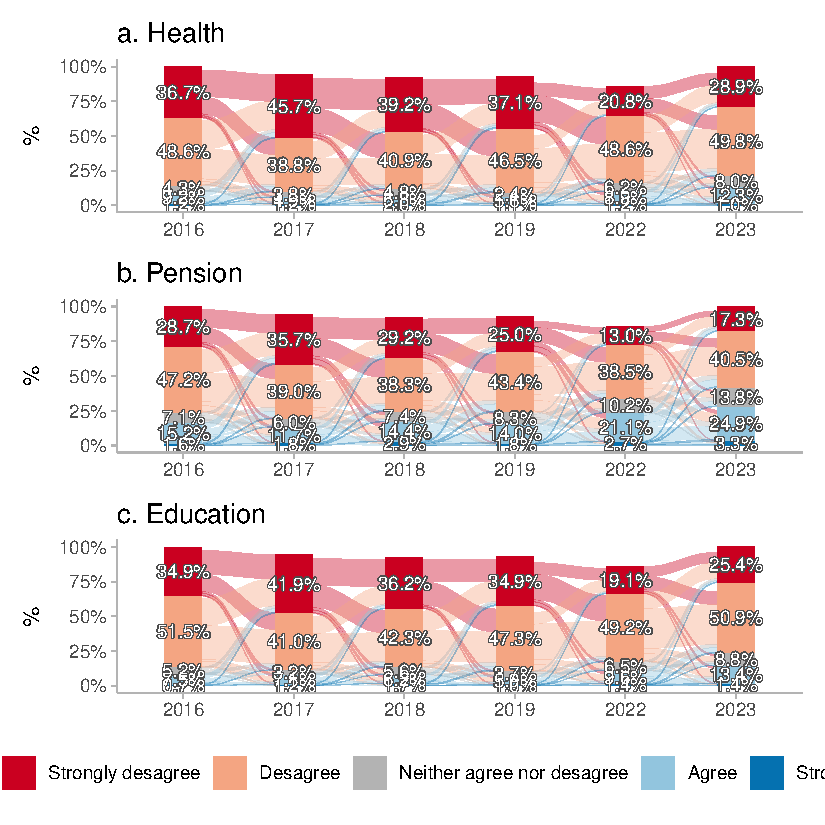
\includegraphics[width=1\textwidth,height=\textheight]{02-analysis_files/figure-pdf/fig-alluvial-1.pdf}

}

\end{figure}%

\subsection{Correlations}\label{correlations}

\begin{Shaded}
\begin{Highlighting}[]
\NormalTok{df\_study1\_long\_t7 }\SpecialCharTok{\%\textgreater{}\%}
  \FunctionTok{filter}\NormalTok{(ola }\SpecialCharTok{==} \DecValTok{7}\NormalTok{) }\SpecialCharTok{\%\textgreater{}\%} 
  \FunctionTok{select}\NormalTok{(mjp, perc\_inequality, just\_inequality, merit\_effort, merit\_talent) }\SpecialCharTok{\%\textgreater{}\%} 
  \FunctionTok{mutate\_all}\NormalTok{(}\AttributeTok{.funs =} \SpecialCharTok{\textasciitilde{}} \FunctionTok{as.numeric}\NormalTok{(.)) }\SpecialCharTok{\%\textgreater{}\%} 
\NormalTok{  sjPlot}\SpecialCharTok{::}\FunctionTok{tab\_corr}\NormalTok{(., }\AttributeTok{triangle =} \StringTok{"lower"}\NormalTok{)}
\end{Highlighting}
\end{Shaded}

\begin{longtable}[]{@{}llllll@{}}
\toprule\noalign{}
\endhead
\bottomrule\noalign{}
\endlastfoot
~ & mjp & perc\_inequality & just\_inequality & merit\_effort &
merit\_talent \\
mjp & ~ & ~ & ~ & ~ & ~ \\
perc\_inequality & -0.049{} & ~ & ~ & ~ & ~ \\
just\_inequality & 0.162{***} & 0.524{***} & ~ & ~ & ~ \\
merit\_effort & 0.140{***} & -0.041{} & 0.046{} & ~ & ~ \\
merit\_talent & 0.117{***} & -0.039{} & 0.062{*} & 0.688{***} & ~ \\
\multicolumn{6}{@{}r@{}}{%
Computed correlation used pearson-method with listwise-deletion.} \\
\end{longtable}

\subsection{Longitudinal multilevel
models}\label{longitudinal-multilevel-models}

\begin{Shaded}
\begin{Highlighting}[]
\CommentTok{\# Generate analytical sample}

\NormalTok{df\_study1 }\OtherTok{\textless{}{-}}\NormalTok{ df\_study1\_long\_t7 }\SpecialCharTok{\%\textgreater{}\%}
  \FunctionTok{select}\NormalTok{(idencuesta,}
\NormalTok{         ola,}
\NormalTok{         ponderador\_long\_total,}
\NormalTok{         mjp, }
\NormalTok{         perc\_inequality, }
\NormalTok{         just\_inequality,}
\NormalTok{         merit\_effort, }
\NormalTok{         merit\_talent, }
\NormalTok{         educ,}
\NormalTok{         quintil1,}
\NormalTok{         sex,}
\NormalTok{         age,}
\NormalTok{         ess, }
\NormalTok{         ideo) }\SpecialCharTok{\%\textgreater{}\%} 
  \FunctionTok{na.omit}\NormalTok{() }\SpecialCharTok{\%\textgreater{}\%} 
  \FunctionTok{mutate}\NormalTok{(}\AttributeTok{ola =} \FunctionTok{as.factor}\NormalTok{(ola),}
         \AttributeTok{ola\_num =} \FunctionTok{as.numeric}\NormalTok{(ola),}
         \AttributeTok{ola\_2=}\FunctionTok{as.numeric}\NormalTok{(ola)}\SpecialCharTok{\^{}}\DecValTok{2}\NormalTok{)}

\NormalTok{df\_study1 }\OtherTok{\textless{}{-}}\NormalTok{ df\_study1 }\SpecialCharTok{\%\textgreater{}\%}
  \FunctionTok{group\_by}\NormalTok{(idencuesta) }\SpecialCharTok{\%\textgreater{}\%}             \CommentTok{\# Agrupar por el identificador del participante}
  \FunctionTok{mutate}\NormalTok{(}\AttributeTok{n\_participaciones =} \FunctionTok{n}\NormalTok{()) }\SpecialCharTok{\%\textgreater{}\%}  \CommentTok{\# Contar el número de filas (participaciones) por participante}
  \FunctionTok{ungroup}\NormalTok{()}

\NormalTok{df\_study1 }\OtherTok{\textless{}{-}}\NormalTok{ df\_study1 }\SpecialCharTok{\%\textgreater{}\%} \FunctionTok{filter}\NormalTok{(n\_participaciones}\SpecialCharTok{\textgreater{}}\DecValTok{1}\NormalTok{)}

\NormalTok{df\_study1}\SpecialCharTok{$}\NormalTok{merit\_effort }\OtherTok{\textless{}{-}} \FunctionTok{as\_numeric}\NormalTok{(df\_study1}\SpecialCharTok{$}\NormalTok{merit\_effort)}
\NormalTok{df\_study1}\SpecialCharTok{$}\NormalTok{merit\_talent }\OtherTok{\textless{}{-}} \FunctionTok{as\_numeric}\NormalTok{(df\_study1}\SpecialCharTok{$}\NormalTok{merit\_talent)}

\NormalTok{df\_study1 }\OtherTok{\textless{}{-}}\NormalTok{ df\_study1 }\SpecialCharTok{\%\textgreater{}\%} 
  \FunctionTok{mutate}\NormalTok{(}\AttributeTok{ola =} \FunctionTok{case\_when}\NormalTok{(ola }\SpecialCharTok{==} \DecValTok{1} \SpecialCharTok{\textasciitilde{}} \StringTok{"2016"}\NormalTok{,}
\NormalTok{                         ola }\SpecialCharTok{==} \DecValTok{2} \SpecialCharTok{\textasciitilde{}} \StringTok{"2017"}\NormalTok{,}
\NormalTok{                         ola }\SpecialCharTok{==} \DecValTok{3} \SpecialCharTok{\textasciitilde{}} \StringTok{"2018"}\NormalTok{,}
\NormalTok{                         ola }\SpecialCharTok{==} \DecValTok{4} \SpecialCharTok{\textasciitilde{}} \StringTok{"2019"}\NormalTok{,}
\NormalTok{                         ola }\SpecialCharTok{==} \DecValTok{6} \SpecialCharTok{\textasciitilde{}} \StringTok{"2022"}\NormalTok{,}
\NormalTok{                         ola }\SpecialCharTok{==} \DecValTok{7} \SpecialCharTok{\textasciitilde{}} \StringTok{"2023"}\NormalTok{),}
         \AttributeTok{ola =} \FunctionTok{factor}\NormalTok{(ola, }\AttributeTok{levels =} \FunctionTok{c}\NormalTok{(}\StringTok{"2016"}\NormalTok{,}
                                        \StringTok{"2017"}\NormalTok{,}
                                        \StringTok{"2018"}\NormalTok{,}
                                        \StringTok{"2019"}\NormalTok{,}
                                        \StringTok{"2022"}\NormalTok{,}
                                        \StringTok{"2023"}\NormalTok{)))}


\NormalTok{df\_study1 }\OtherTok{\textless{}{-}}\NormalTok{ df\_study1 }\SpecialCharTok{\%\textgreater{}\%} 
  \FunctionTok{group\_by}\NormalTok{(idencuesta) }\SpecialCharTok{\%\textgreater{}\%} 
  \FunctionTok{mutate}\NormalTok{(}\AttributeTok{perc\_inequality\_mean =} \FunctionTok{mean}\NormalTok{(perc\_inequality, }\AttributeTok{na.rm =}\NormalTok{ T),}
         \AttributeTok{perc\_inequality\_cwc =}\NormalTok{ perc\_inequality }\SpecialCharTok{{-}}\NormalTok{ perc\_inequality\_mean,}
         \AttributeTok{just\_inequality\_mean =} \FunctionTok{mean}\NormalTok{(just\_inequality, }\AttributeTok{na.rm =}\NormalTok{ T),}
         \AttributeTok{just\_inequality\_cwc =}\NormalTok{ just\_inequality }\SpecialCharTok{{-}}\NormalTok{ just\_inequality\_mean,}
         \AttributeTok{merit\_effort\_mean =} \FunctionTok{mean}\NormalTok{(merit\_effort, }\AttributeTok{na.rm =}\NormalTok{ T),}
         \AttributeTok{merit\_effort\_cwc =}\NormalTok{ merit\_effort }\SpecialCharTok{{-}}\NormalTok{ merit\_effort\_mean,}
         \AttributeTok{merit\_talent\_mean =} \FunctionTok{mean}\NormalTok{(merit\_talent, }\AttributeTok{na.rm =}\NormalTok{ T),}
         \AttributeTok{merit\_talent\_cwc =}\NormalTok{ merit\_talent }\SpecialCharTok{{-}}\NormalTok{ merit\_talent\_mean,}
\NormalTok{         ) }\SpecialCharTok{\%\textgreater{}\%} 
  \FunctionTok{ungroup}\NormalTok{()}
\end{Highlighting}
\end{Shaded}

\begin{Shaded}
\begin{Highlighting}[]
\NormalTok{m0 }\OtherTok{\textless{}{-}} \FunctionTok{lmer}\NormalTok{(mjp }\SpecialCharTok{\textasciitilde{}} \DecValTok{1} \SpecialCharTok{+}\NormalTok{ (}\DecValTok{1} \SpecialCharTok{|}\NormalTok{ idencuesta), }
                \AttributeTok{data =}\NormalTok{ df\_study1)}

\NormalTok{performance}\SpecialCharTok{::}\FunctionTok{icc}\NormalTok{(m0, }\AttributeTok{by\_group =}\NormalTok{ T)}
\end{Highlighting}
\end{Shaded}

\begin{verbatim}
# ICC by Group

Group      |   ICC
------------------
idencuesta | 0.232
\end{verbatim}

\begin{Shaded}
\begin{Highlighting}[]
\NormalTok{m1 }\OtherTok{\textless{}{-}} \FunctionTok{lmer}\NormalTok{(mjp }\SpecialCharTok{\textasciitilde{}} \DecValTok{1} \SpecialCharTok{+}\NormalTok{ ola }\SpecialCharTok{+}\NormalTok{ (}\DecValTok{1} \SpecialCharTok{|}\NormalTok{ idencuesta),}
                \AttributeTok{data =}\NormalTok{ df\_study1)}

\NormalTok{m1}\FloatTok{.1} \OtherTok{\textless{}{-}} \FunctionTok{lmer}\NormalTok{(mjp }\SpecialCharTok{\textasciitilde{}} \DecValTok{1} \SpecialCharTok{+}\NormalTok{ ola\_num }\SpecialCharTok{+}\NormalTok{ ola\_2 }\SpecialCharTok{+}\NormalTok{ (}\DecValTok{1} \SpecialCharTok{|}\NormalTok{ idencuesta),}
                \AttributeTok{data =}\NormalTok{ df\_study1)}

\NormalTok{m2 }\OtherTok{\textless{}{-}} \FunctionTok{lmer}\NormalTok{(mjp }\SpecialCharTok{\textasciitilde{}} \DecValTok{1} \SpecialCharTok{+}\NormalTok{ ola\_num }\SpecialCharTok{+}\NormalTok{ ola\_2 }\SpecialCharTok{+}\NormalTok{ (}\DecValTok{1} \SpecialCharTok{+}\NormalTok{ ola\_num }\SpecialCharTok{|}\NormalTok{ idencuesta),}
                \AttributeTok{data =}\NormalTok{ df\_study1)}

\FunctionTok{anova}\NormalTok{(m1}\FloatTok{.1}\NormalTok{, m2)}
\end{Highlighting}
\end{Shaded}

\begin{verbatim}
Data: df_study1
Models:
m1.1: mjp ~ 1 + ola_num + ola_2 + (1 | idencuesta)
m2: mjp ~ 1 + ola_num + ola_2 + (1 + ola_num | idencuesta)
     npar   AIC   BIC logLik deviance  Chisq Df           Pr(>Chisq)    
m1.1    5 20352 20387 -10171    20342                                   
m2      7 20288 20338 -10137    20274 67.966  2 0.000000000000001743 ***
---
Signif. codes:  0 '***' 0.001 '**' 0.01 '*' 0.05 '.' 0.1 ' ' 1
\end{verbatim}

\begin{Shaded}
\begin{Highlighting}[]
\NormalTok{m3 }\OtherTok{\textless{}{-}} \FunctionTok{lmer}\NormalTok{(mjp }\SpecialCharTok{\textasciitilde{}} \DecValTok{1} \SpecialCharTok{+}\NormalTok{ ola\_num }\SpecialCharTok{+}\NormalTok{ ola\_2 }\SpecialCharTok{+}\NormalTok{ perc\_inequality }\SpecialCharTok{+}\NormalTok{ (}\DecValTok{1} \SpecialCharTok{+}\NormalTok{ ola\_num }\SpecialCharTok{|}\NormalTok{ idencuesta), }
           \AttributeTok{data =}\NormalTok{ df\_study1)}

\NormalTok{m4 }\OtherTok{\textless{}{-}} \FunctionTok{lmer}\NormalTok{(mjp }\SpecialCharTok{\textasciitilde{}} \DecValTok{1} \SpecialCharTok{+}\NormalTok{ ola\_num }\SpecialCharTok{+}\NormalTok{ ola\_2 }\SpecialCharTok{+}\NormalTok{ perc\_inequality }\SpecialCharTok{+}\NormalTok{ just\_inequality }\SpecialCharTok{+}\NormalTok{ (}\DecValTok{1} \SpecialCharTok{+}\NormalTok{ ola\_num }\SpecialCharTok{|}\NormalTok{ idencuesta),}
                \AttributeTok{data =}\NormalTok{ df\_study1)}

\NormalTok{m5 }\OtherTok{\textless{}{-}} \FunctionTok{lmer}\NormalTok{(mjp }\SpecialCharTok{\textasciitilde{}} \DecValTok{1} \SpecialCharTok{+}\NormalTok{ ola\_num }\SpecialCharTok{+}\NormalTok{ ola\_2 }\SpecialCharTok{+}\NormalTok{ perc\_inequality }\SpecialCharTok{+}\NormalTok{ just\_inequality }\SpecialCharTok{+}\NormalTok{ merit\_effort }\SpecialCharTok{+}\NormalTok{ (}\DecValTok{1} \SpecialCharTok{+}\NormalTok{ ola\_num }\SpecialCharTok{|}\NormalTok{ idencuesta),}
                \AttributeTok{data =}\NormalTok{ df\_study1)}

\NormalTok{m6 }\OtherTok{\textless{}{-}} \FunctionTok{lmer}\NormalTok{(mjp }\SpecialCharTok{\textasciitilde{}} \DecValTok{1} \SpecialCharTok{+}\NormalTok{ ola\_num }\SpecialCharTok{+}\NormalTok{ ola\_2 }\SpecialCharTok{+}\NormalTok{ perc\_inequality }\SpecialCharTok{+}\NormalTok{ just\_inequality }\SpecialCharTok{+}\NormalTok{ merit\_effort }\SpecialCharTok{+}\NormalTok{ merit\_talent }\SpecialCharTok{+}\NormalTok{ (}\DecValTok{1} \SpecialCharTok{+}\NormalTok{ ola\_num }\SpecialCharTok{|}\NormalTok{ idencuesta),}
                \AttributeTok{data =}\NormalTok{ df\_study1)}


\NormalTok{m7 }\OtherTok{\textless{}{-}} \FunctionTok{lmer}\NormalTok{(mjp }\SpecialCharTok{\textasciitilde{}} \DecValTok{1} \SpecialCharTok{+}\NormalTok{ ola\_num }\SpecialCharTok{+}\NormalTok{ ola\_2 }\SpecialCharTok{+}\NormalTok{ perc\_inequality }\SpecialCharTok{+}\NormalTok{ just\_inequality }\SpecialCharTok{+}\NormalTok{ merit\_effort }\SpecialCharTok{+}\NormalTok{ merit\_talent }\SpecialCharTok{+}\NormalTok{ perc\_inequality\_mean }\SpecialCharTok{+}\NormalTok{ just\_inequality\_mean }\SpecialCharTok{+}\NormalTok{ merit\_effort\_mean }\SpecialCharTok{+}\NormalTok{ merit\_talent\_mean }\SpecialCharTok{+}\NormalTok{ (}\DecValTok{1} \SpecialCharTok{+}\NormalTok{ ola\_num }\SpecialCharTok{|}\NormalTok{ idencuesta),}
                \AttributeTok{data =}\NormalTok{ df\_study1)}

\NormalTok{m8 }\OtherTok{\textless{}{-}} \FunctionTok{lmer}\NormalTok{(mjp }\SpecialCharTok{\textasciitilde{}} \DecValTok{1} \SpecialCharTok{+}\NormalTok{ ola\_num }\SpecialCharTok{+}\NormalTok{ ola\_2 }\SpecialCharTok{+}\NormalTok{ perc\_inequality }\SpecialCharTok{+}\NormalTok{ just\_inequality }\SpecialCharTok{+}\NormalTok{ merit\_effort }\SpecialCharTok{+}\NormalTok{ merit\_talent }\SpecialCharTok{+}\NormalTok{ perc\_inequality\_mean }\SpecialCharTok{+}\NormalTok{ just\_inequality\_mean }\SpecialCharTok{+}\NormalTok{ merit\_effort\_mean }\SpecialCharTok{+}\NormalTok{ merit\_talent\_mean }\SpecialCharTok{+}\NormalTok{ educ }\SpecialCharTok{+}\NormalTok{ quintil1 }\SpecialCharTok{+}\NormalTok{ ess }\SpecialCharTok{+}\NormalTok{ ideo }\SpecialCharTok{+}\NormalTok{ sex }\SpecialCharTok{+}\NormalTok{ age }\SpecialCharTok{+}\NormalTok{ (}\DecValTok{1} \SpecialCharTok{+}\NormalTok{ ola\_num }\SpecialCharTok{|}\NormalTok{ idencuesta),}
                \AttributeTok{data =}\NormalTok{ df\_study1)}

\NormalTok{m9 }\OtherTok{\textless{}{-}} \FunctionTok{lmer}\NormalTok{(mjp }\SpecialCharTok{\textasciitilde{}} \DecValTok{1} \SpecialCharTok{+}\NormalTok{ ola\_num }\SpecialCharTok{+}\NormalTok{ ola\_2 }\SpecialCharTok{+}\NormalTok{ perc\_inequality}\SpecialCharTok{*}\NormalTok{ola\_num }\SpecialCharTok{+}\NormalTok{ just\_inequality }\SpecialCharTok{+}\NormalTok{ merit\_effort }\SpecialCharTok{+}\NormalTok{ merit\_talent }\SpecialCharTok{+}\NormalTok{ perc\_inequality\_mean }\SpecialCharTok{+}\NormalTok{ just\_inequality\_mean }\SpecialCharTok{+}\NormalTok{ merit\_effort\_mean }\SpecialCharTok{+}\NormalTok{ merit\_talent\_mean }\SpecialCharTok{+}\NormalTok{ educ }\SpecialCharTok{+}\NormalTok{ quintil1 }\SpecialCharTok{+}\NormalTok{ ess }\SpecialCharTok{+}\NormalTok{ ideo }\SpecialCharTok{+}\NormalTok{ sex }\SpecialCharTok{+}\NormalTok{ age }\SpecialCharTok{+}\NormalTok{ (}\DecValTok{1} \SpecialCharTok{+}\NormalTok{ ola\_num }\SpecialCharTok{|}\NormalTok{ idencuesta),}
                \AttributeTok{data =}\NormalTok{ df\_study1)}

\NormalTok{m10 }\OtherTok{\textless{}{-}} \FunctionTok{lmer}\NormalTok{(mjp }\SpecialCharTok{\textasciitilde{}} \DecValTok{1} \SpecialCharTok{+}\NormalTok{ ola\_num }\SpecialCharTok{+}\NormalTok{ ola\_2 }\SpecialCharTok{+}\NormalTok{ perc\_inequality}\SpecialCharTok{*}\NormalTok{ola\_num }\SpecialCharTok{+}\NormalTok{ just\_inequality}\SpecialCharTok{*}\NormalTok{ola\_num }\SpecialCharTok{+}\NormalTok{ merit\_effort }\SpecialCharTok{+}\NormalTok{ merit\_talent }\SpecialCharTok{+}\NormalTok{ perc\_inequality\_mean }\SpecialCharTok{+}\NormalTok{ just\_inequality\_mean }\SpecialCharTok{+}\NormalTok{ merit\_effort\_mean }\SpecialCharTok{+}\NormalTok{ merit\_talent\_mean }\SpecialCharTok{+}\NormalTok{ educ }\SpecialCharTok{+}\NormalTok{ quintil1 }\SpecialCharTok{+}\NormalTok{ ess }\SpecialCharTok{+}\NormalTok{ ideo }\SpecialCharTok{+}\NormalTok{ sex }\SpecialCharTok{+}\NormalTok{ age }\SpecialCharTok{+}\NormalTok{ (}\DecValTok{1} \SpecialCharTok{+}\NormalTok{ ola\_num }\SpecialCharTok{|}\NormalTok{ idencuesta),}
                \AttributeTok{data =}\NormalTok{ df\_study1)}

\NormalTok{m11 }\OtherTok{\textless{}{-}} \FunctionTok{lmer}\NormalTok{(mjp }\SpecialCharTok{\textasciitilde{}} \DecValTok{1} \SpecialCharTok{+}\NormalTok{ ola\_num }\SpecialCharTok{+}\NormalTok{ ola\_2 }\SpecialCharTok{+}\NormalTok{ perc\_inequality}\SpecialCharTok{*}\NormalTok{ola\_num }\SpecialCharTok{+}\NormalTok{ just\_inequality}\SpecialCharTok{*}\NormalTok{ola\_num }\SpecialCharTok{+}\NormalTok{ merit\_effort}\SpecialCharTok{*}\NormalTok{ola\_num }\SpecialCharTok{+}\NormalTok{ merit\_talent }\SpecialCharTok{+}\NormalTok{ perc\_inequality\_mean }\SpecialCharTok{+}\NormalTok{ just\_inequality\_mean }\SpecialCharTok{+}\NormalTok{ merit\_effort\_mean }\SpecialCharTok{+}\NormalTok{ merit\_talent\_mean }\SpecialCharTok{+}\NormalTok{ educ }\SpecialCharTok{+}\NormalTok{ quintil1 }\SpecialCharTok{+}\NormalTok{ ess }\SpecialCharTok{+}\NormalTok{ ideo }\SpecialCharTok{+}\NormalTok{ sex }\SpecialCharTok{+}\NormalTok{ age }\SpecialCharTok{+}\NormalTok{ (}\DecValTok{1} \SpecialCharTok{+}\NormalTok{ ola\_num }\SpecialCharTok{|}\NormalTok{ idencuesta),}
                \AttributeTok{data =}\NormalTok{ df\_study1)}

\NormalTok{m12 }\OtherTok{\textless{}{-}} \FunctionTok{lmer}\NormalTok{(mjp }\SpecialCharTok{\textasciitilde{}} \DecValTok{1} \SpecialCharTok{+}\NormalTok{ ola\_num }\SpecialCharTok{+}\NormalTok{ ola\_2 }\SpecialCharTok{+}\NormalTok{ perc\_inequality}\SpecialCharTok{*}\NormalTok{ola\_num }\SpecialCharTok{+}\NormalTok{ just\_inequality}\SpecialCharTok{*}\NormalTok{ola\_num }\SpecialCharTok{+}\NormalTok{ merit\_effort}\SpecialCharTok{*}\NormalTok{ola\_num }\SpecialCharTok{+}\NormalTok{ merit\_talent}\SpecialCharTok{*}\NormalTok{ola\_num }\SpecialCharTok{+}\NormalTok{ perc\_inequality\_mean }\SpecialCharTok{+}\NormalTok{ just\_inequality\_mean }\SpecialCharTok{+}\NormalTok{ merit\_effort\_mean }\SpecialCharTok{+}\NormalTok{ merit\_talent\_mean }\SpecialCharTok{+}\NormalTok{ educ }\SpecialCharTok{+}\NormalTok{ quintil1 }\SpecialCharTok{+}\NormalTok{ ess }\SpecialCharTok{+}\NormalTok{ ideo }\SpecialCharTok{+}\NormalTok{ sex }\SpecialCharTok{+}\NormalTok{ age }\SpecialCharTok{+}\NormalTok{ (}\DecValTok{1} \SpecialCharTok{+}\NormalTok{ ola\_num }\SpecialCharTok{|}\NormalTok{ idencuesta),}
                \AttributeTok{data =}\NormalTok{ df\_study1)}
\end{Highlighting}
\end{Shaded}

\begin{table}

\caption{\label{tbl-modelos}Longitudinal multilevel models for market
justice preferences}

\centering{

\begin{Shaded}
\begin{Highlighting}[]
\NormalTok{ccoef }\OtherTok{\textless{}{-}} \FunctionTok{list}\NormalTok{(}
  \StringTok{"(Intercept)"} \OtherTok{=} \StringTok{"Intercept"}\NormalTok{,}
  \StringTok{"ola2017"} \OtherTok{=} \StringTok{"Wave 2017"}\NormalTok{,}
  \StringTok{"ola2018"} \OtherTok{=} \StringTok{"Wave 2018"}\NormalTok{,}
  \StringTok{"ola2019"} \OtherTok{=} \StringTok{"Wave 2019"}\NormalTok{,}
  \StringTok{"ola2022"} \OtherTok{=} \StringTok{"Wave 2022"}\NormalTok{,}
  \StringTok{"ola2023"} \OtherTok{=} \StringTok{"Wave 2023"}\NormalTok{,}
  \AttributeTok{ola\_num =} \StringTok{"Wave"}\NormalTok{,}
  \AttributeTok{ola\_2 =} \StringTok{"Wave\^{}2"}\NormalTok{,}
  \AttributeTok{perc\_inequality =} \StringTok{"Perception inequality (WE)"}\NormalTok{,}
  \AttributeTok{just\_inequality =} \StringTok{"Justification inequality (WE)"}\NormalTok{,}
  \AttributeTok{merit\_effort =} \StringTok{"Merit: Effort (WE)"}\NormalTok{,}
  \AttributeTok{merit\_talent =} \StringTok{"Merit: Talent (WE)"}\NormalTok{,}
  \AttributeTok{perc\_inequality\_mean =} \StringTok{"Perception inequality (BE)"}\NormalTok{,}
  \AttributeTok{just\_inequality\_mean =} \StringTok{"Justification inequality (BE)"}\NormalTok{,}
  \AttributeTok{merit\_effort\_mean =} \StringTok{"Merit: Effort (BE)"}\NormalTok{,}
  \AttributeTok{merit\_talent\_mean =} \StringTok{"Merit: Talent (BE)"}\NormalTok{,}
  \AttributeTok{educUniversitary =} \StringTok{"Universitary (Ref.= Less than universitary)"}\NormalTok{,}
  \AttributeTok{quintil1Q2 =} \StringTok{"Quintile 2"}\NormalTok{,}
  \AttributeTok{quintil1Q3 =} \StringTok{"Quintile 3"}\NormalTok{,}
  \AttributeTok{quintil1Q4 =} \StringTok{"Quintile 4"}\NormalTok{,}
  \AttributeTok{quintil1Q5 =} \StringTok{"Quintile 5"}\NormalTok{,}
  \AttributeTok{quintil1QNA =} \StringTok{"Quintile NA"}\NormalTok{,}
  \AttributeTok{ess =} \StringTok{"Subjective social status"}\NormalTok{,}
  \AttributeTok{ideoCenter =} \StringTok{"Center"}\NormalTok{,}
  \AttributeTok{ideoRight =} \StringTok{"Right"}\NormalTok{,}
  \StringTok{"ideoDoes not identify"} \OtherTok{=} \StringTok{"Does not identify"}\NormalTok{,}
  \AttributeTok{sexFemale =} \StringTok{"Female (Ref.= Male)"}\NormalTok{,}
  \StringTok{"age30{-}49"} \OtherTok{=} \StringTok{"30{-}49"}\NormalTok{,}
  \StringTok{"age50{-}64"} \OtherTok{=} \StringTok{"50{-}64"}\NormalTok{,}
  \StringTok{"age65 or more"} \OtherTok{=} \StringTok{"65 or more"}
\NormalTok{  )}

\NormalTok{texreg}\SpecialCharTok{::}\FunctionTok{htmlreg}\NormalTok{(}\FunctionTok{list}\NormalTok{(m1, m2, m3, m4, m5, m6, m7, m8),}
               \AttributeTok{custom.model.names =} \FunctionTok{c}\NormalTok{(}\FunctionTok{paste0}\NormalTok{(}\StringTok{"Model "}\NormalTok{, }\FunctionTok{seq}\NormalTok{(}\DecValTok{1}\SpecialCharTok{:}\DecValTok{8}\NormalTok{))),}
               \AttributeTok{caption =} \ConstantTok{NULL}\NormalTok{,}
               \AttributeTok{stars =} \FunctionTok{c}\NormalTok{(}\FloatTok{0.05}\NormalTok{, }\FloatTok{0.01}\NormalTok{, }\FloatTok{0.001}\NormalTok{),}
               \AttributeTok{custom.coef.map =}\NormalTok{ ccoef,}
               \AttributeTok{digits =} \DecValTok{3}\NormalTok{,}
               \AttributeTok{groups =} \FunctionTok{list}\NormalTok{(}\StringTok{"Wave (Ref.= 2016)"} \OtherTok{=} \DecValTok{2}\SpecialCharTok{:}\DecValTok{6}\NormalTok{, }\StringTok{"Income (Ref.= Quintile 1)"} \OtherTok{=} \DecValTok{18}\SpecialCharTok{:}\DecValTok{22}\NormalTok{, }\StringTok{"Political identification (Ref.= Left)"} \OtherTok{=} \DecValTok{24}\SpecialCharTok{:}\DecValTok{26}\NormalTok{, }\StringTok{"Age (Ref. = 18{-}29)"} \OtherTok{=} \DecValTok{28}\SpecialCharTok{:}\DecValTok{30}\NormalTok{),}
               \AttributeTok{custom.note =} \StringTok{"Note: Cells contain regression coefficients with standard errors in parentheses. \%stars."}\NormalTok{,}
               \AttributeTok{threeparttable =}\NormalTok{ T,}
               \AttributeTok{leading.zero =}\NormalTok{ T,}
               \AttributeTok{float.pos =} \StringTok{"h!"}\NormalTok{,}
               \AttributeTok{use.packages =}\NormalTok{ F,}
               \AttributeTok{booktabs =}\NormalTok{ T,}
               \AttributeTok{scalebox =} \DecValTok{1}\NormalTok{)}
\end{Highlighting}
\end{Shaded}

~

Model 1

Model 2

Model 3

Model 4

Model 5

Model 6

Model 7

Model 8

Intercept

1.966***

1.968***

2.108***

2.063***

1.755***

1.725***

1.537***

1.565***

~

(0.022)

(0.033)

(0.046)

(0.045)

(0.052)

(0.053)

(0.095)

(0.112)

Wave (Ref.= 2016)

~

~

~

~

~

~

~

~

~

~

~

~

~

~

~

~

~

~~~~~Wave 2017

-0.163***

~

~

~

~

~

~

~

~

(0.028)

~

~

~

~

~

~

~

~~~~~Wave 2018

-0.013

~

~

~

~

~

~

~

~

(0.027)

~

~

~

~

~

~

~

~~~~~Wave 2019

-0.043

~

~

~

~

~

~

~

~

(0.027)

~

~

~

~

~

~

~

~~~~~Wave 2022

0.289***

~

~

~

~

~

~

~

~

(0.028)

~

~

~

~

~

~

~

~~~~~Wave 2023

0.284***

~

~

~

~

~

~

~

~

(0.027)

~

~

~

~

~

~

~

Wave

~

-0.069***

-0.072***

-0.057**

-0.057**

-0.058**

-0.064***

-0.064***

~

~

(0.018)

(0.018)

(0.018)

(0.018)

(0.018)

(0.018)

(0.018)

Wave\^{}2

~

0.017***

0.017***

0.015***

0.015***

0.015***

0.016***

0.016***

~

~

(0.002)

(0.002)

(0.002)

(0.002)

(0.002)

(0.002)

(0.002)

Perception inequality (WE)

~

~

-0.038***

-0.087***

-0.076***

-0.076***

-0.058***

-0.058***

~

~

~

(0.009)

(0.010)

(0.010)

(0.010)

(0.011)

(0.011)

Justification inequality (WE)

~

~

~

0.101***

0.096***

0.095***

0.056***

0.056***

~

~

~

~

(0.009)

(0.009)

(0.009)

(0.010)

(0.010)

Merit: Effort (WE)

~

~

~

~

0.107***

0.088***

0.071***

0.071***

~

~

~

~

~

(0.009)

(0.011)

(0.012)

(0.012)

Merit: Talent (WE)

~

~

~

~

~

0.028*

0.025*

0.024*

~

~

~

~

~

~

(0.011)

(0.012)

(0.012)

Perception inequality (BE)

~

~

~

~

~

~

-0.077***

-0.078***

~

~

~

~

~

~

~

(0.023)

(0.023)

Justification inequality (BE)

~

~

~

~

~

~

0.159***

0.134***

~

~

~

~

~

~

~

(0.021)

(0.021)

Merit: Effort (BE)

~

~

~

~

~

~

0.095**

0.091**

~

~

~

~

~

~

~

(0.033)

(0.033)

Merit: Talent (BE)

~

~

~

~

~

~

-0.008

-0.017

~

~

~

~

~

~

~

(0.033)

(0.033)

Universitary (Ref.= Less than universitary)

~

~

~

~

~

~

~

-0.006

~

~

~

~

~

~

~

~

(0.035)

Income (Ref.= Quintile 1)

~

~

~

~

~

~

~

~

~

~

~

~

~

~

~

~

~

~~~~~Quintile 2

~

~

~

~

~

~

~

0.002

~

~

~

~

~

~

~

~

(0.038)

~~~~~Quintile 3

~

~

~

~

~

~

~

0.035

~

~

~

~

~

~

~

~

(0.038)

~~~~~Quintile 4

~

~

~

~

~

~

~

0.097*

~

~

~

~

~

~

~

~

(0.039)

~~~~~Quintile 5

~

~

~

~

~

~

~

0.147***

~

~

~

~

~

~

~

~

(0.042)

~~~~~Quintile NA

~

~

~

~

~

~

~

0.173**

~

~

~

~

~

~

~

~

(0.066)

Subjective social status

~

~

~

~

~

~

~

-0.007

~

~

~

~

~

~

~

~

(0.008)

Political identification (Ref.= Left)

~

~

~

~

~

~

~

~

~

~

~

~

~

~

~

~

~

~~~~~Center

~

~

~

~

~

~

~

0.057

~

~

~

~

~

~

~

~

(0.037)

~~~~~Right

~

~

~

~

~

~

~

0.245***

~

~

~

~

~

~

~

~

(0.042)

~~~~~Does not identify

~

~

~

~

~

~

~

0.095**

~

~

~

~

~

~

~

~

(0.032)

Female (Ref.= Male)

~

~

~

~

~

~

~

-0.081**

~

~

~

~

~

~

~

~

(0.026)

Age (Ref. = 18-29)

~

~

~

~

~

~

~

~

~

~

~

~

~

~

~

~

~

~~~~~30-49

~

~

~

~

~

~

~

-0.009

~

~

~

~

~

~

~

~

(0.037)

~~~~~50-64

~

~

~

~

~

~

~

0.003

~

~

~

~

~

~

~

~

(0.039)

~~~~~65 or more

~

~

~

~

~

~

~

0.002

~

~

~

~

~

~

~

~

(0.046)

AIC

20324.667

20314.582

20304.765

20190.877

20051.570

20054.362

20003.452

20033.225

BIC

20381.029

20363.898

20361.127

20254.284

20122.022

20131.859

20109.130

20237.537

Log Likelihood

-10154.334

-10150.291

-10144.383

-10086.439

-10015.785

-10016.181

-9986.726

-9987.613

Num. obs.

8478

8478

8478

8478

8478

8478

8478

8478

Num. groups: idencuesta

1682

1682

1682

1682

1682

1682

1682

1682

Var: idencuesta (Intercept)

0.176

0.218

0.213

0.206

0.181

0.180

0.182

0.173

Var: Residual

0.528

0.495

0.494

0.493

0.491

0.490

0.488

0.488

Var: idencuesta ola\_num

~

0.007

0.007

0.007

0.006

0.006

0.006

0.006

Cov: idencuesta (Intercept) ola\_num

~

-0.018

-0.017

-0.018

-0.015

-0.015

-0.016

-0.016

Note: Cells contain regression coefficients with standard errors in
parentheses. ***p \textless{} 0.001; **p \textless{} 0.01; *p
\textless{} 0.05.

}

\end{table}%

\begin{table}

\caption{\label{tbl-interactions}Time interactions within effects for
market justice preferences}

\centering{

\begin{Shaded}
\begin{Highlighting}[]
\NormalTok{ccoef }\OtherTok{\textless{}{-}} \FunctionTok{list}\NormalTok{(}
  \StringTok{"(Intercept)"} \OtherTok{=} \StringTok{"Intercept"}\NormalTok{,}
  \StringTok{"ola\_num:perc\_inequality"} \OtherTok{=} \StringTok{"Perception inequality (WE) x Wave"}\NormalTok{,}
  \StringTok{"ola\_num:just\_inequality"} \OtherTok{=} \StringTok{"Justification inequality (WE) x Wave"}\NormalTok{,}
  \StringTok{"ola\_num:merit\_effort"} \OtherTok{=} \StringTok{"Merit: Effort (WE) x Wave"}\NormalTok{,}
  \StringTok{"ola\_num:merit\_talent"} \OtherTok{=} \StringTok{"Merit: Talent (WE) x Wave"}
\NormalTok{  )}

\NormalTok{texreg}\SpecialCharTok{::}\FunctionTok{htmlreg}\NormalTok{(}\FunctionTok{list}\NormalTok{(m9,m10,m11,m12),}
               \AttributeTok{custom.model.names =} \FunctionTok{c}\NormalTok{(}\FunctionTok{paste0}\NormalTok{(}\StringTok{"Model "}\NormalTok{, }\FunctionTok{seq}\NormalTok{(}\DecValTok{9}\SpecialCharTok{:}\DecValTok{12}\NormalTok{))),}
               \AttributeTok{caption =} \ConstantTok{NULL}\NormalTok{,}
               \AttributeTok{stars =} \FunctionTok{c}\NormalTok{(}\FloatTok{0.05}\NormalTok{, }\FloatTok{0.01}\NormalTok{, }\FloatTok{0.001}\NormalTok{),}
               \AttributeTok{custom.coef.map =}\NormalTok{ ccoef,}
               \AttributeTok{digits =} \DecValTok{3}\NormalTok{,}
               \AttributeTok{custom.note =} \StringTok{"Note: Cells contain regression coefficients with standard errors in parentheses. \%stars."}\NormalTok{,}
               \AttributeTok{threeparttable =}\NormalTok{ T,}
               \AttributeTok{leading.zero =}\NormalTok{ T,}
               \AttributeTok{float.pos =} \StringTok{"h!"}\NormalTok{,}
               \AttributeTok{use.packages =}\NormalTok{ F,}
               \AttributeTok{booktabs =}\NormalTok{ T,}
               \AttributeTok{scalebox =} \DecValTok{1}\NormalTok{)}
\end{Highlighting}
\end{Shaded}

~

Model 1

Model 2

Model 3

Model 4

Intercept

1.589***

1.601***

1.472***

1.455***

~

(0.123)

(0.123)

(0.129)

(0.131)

Perception inequality (WE) x Wave

0.002

-0.007

-0.009*

-0.009*

~

(0.004)

(0.004)

(0.004)

(0.004)

Justification inequality (WE) x Wave

~

0.018***

0.018***

0.019***

~

~

(0.004)

(0.004)

(0.004)

Merit: Effort (WE) x Wave

~

~

-0.013**

-0.010

~

~

~

(0.004)

(0.005)

Merit: Talent (WE) x Wave

~

~

~

-0.005

~

~

~

~

(0.005)

AIC

20044.276

20035.653

20036.766

20046.613

BIC

20255.633

20254.055

20262.214

20279.105

Log Likelihood

-9992.138

-9986.826

-9986.383

-9990.306

Num. obs.

8478

8478

8478

8478

Num. groups: idencuesta

1682

1682

1682

1682

Var: idencuesta (Intercept)

0.173

0.168

0.165

0.164

Var: idencuesta ola\_num

0.006

0.006

0.006

0.006

Cov: idencuesta (Intercept) ola\_num

-0.016

-0.015

-0.014

-0.014

Var: Residual

0.488

0.489

0.489

0.489

Note: Cells contain regression coefficients with standard errors in
parentheses. ***p \textless{} 0.001; **p \textless{} 0.01; *p
\textless{} 0.05.

}

\end{table}%



\end{document}
